\begin{document}


\section*{Ejemplos de elementos comúnes en Latex para mejorar el uso de la plantilla}

Esta sección contiene ejemplos de como incluir ciertos elementos comunes en un documento Latex, extraídos del proyecto de \textbf{Elena Allegue Gonzalez}, que donó su documentación para poder hacer esta plantilla de trabajos de fin de grado y que su uso fuese mucho más sencillo. Esta sección contiene ejemplos de dichos elementos basados en lo que ella hizo en su proyecto (la aplicación \textit{GuardMe} \cite{Elena19LNE}, para protección de personas en situaciones de peligro con el móvil), por lo que todos ellos deben ser entendidos en ese contexto. Por favor, no dejes ni esta sección ni ninguno de estos elementos en tu documentación porque son solo ejemplos que tienen sentido en el contexto de su proyecto. Ten en cuenta además que en el cuerpo del propio documento hay algún ejemplo más en la sección en la que corresponde, que debe adaptarse y eliminarse si no es de aplicación.

\subsection*{Paquetes de Latex usados en la plantilla}

\subsubsection*{Paquetes de LaTeX}
Para generar \textbf{documentación en LaTeX} se requiere del \textbf{uso de paquetes}, los cuales son introducidos al mismo mediante el comando \texttt{\textbackslash usepack\\
age\{name\}}, que son instalados en caso de no estarlo ya en el propio editor de texto para su posterior uso.\newline

Se han usado un \textbf{gran número de librerías}, las cuales clasificaré a continuación por tipo de licencia, mencionando en todas ellas su correspondiente autor/autora y funcionalidad:
\begin{itemize}
	\item Licencia MIT
	\begin{itemize}
		\item \texttt{enumitem} sirve para el control de las listas numeradas pudiendo, entre otras, diseñar el tipo de enumerado que aparece en el documento generado. Autor copyright: Javier Be­zos (\url{https://github.com/jbezos/enumitem}).
	\end{itemize}
	\item LaTeX Project Public Li­cense\footnote{La distribución de copias esta permitida, aunque no es posible modificar los documentos bajo esta licencia. LPPL es la licencia que posee el kernel del propio LaTeX además de ser la más común para la distribución sus paquetes.}
	\begin{itemize}
		\item \texttt{nameref} sirve para crear una referencia basada en el nombre del título del capítulo, sección, subsección o lo que corresponda. Autor copyright: Oberdiek Pack­age Sup­port Group.
		\item \texttt{hyperref} sirve para que las referencias, ya sean de tipo \textit{ref} o \textit{nameref} sean clicables y enlazadas con la referencia a la que apuntan, el índice también funciona de esta manera. Además, las urls de sitios web o documentos se abran en el navegador de Internet. Autor copyright: Oberdiek Package Support Group (\url{https://github.com/ho-tex/hyperref}).
		\item \texttt{titlesec} sirve para poder crear diferentes estilos en los títulos de las secciones así como poner estilos concretos a una página. Autor copyright: Javier Be­zos.
		\item \texttt{float} sirve para que una imagen se mantenga en una posición concreta siempre en el documento. LaTeX si no se provee de esta configuración, coloca la imagen donde mejor entre, aunque esto suponga estar en la sección siguiente de donde debería estar. Autor: NaN.(Mantenimiento: Anselm Ling­nau).
		\item \texttt{fancyhdr} se utiliza para el control de los estilos y personalizaciones de posición de los encabezados y pies de páginas de LaTeX. Autor copyright: Piet van Oostrum.
		\item \texttt{enumerate} se utiliza para cambiar el estilo de los marcadores de las listas enumeradas o no.  Autor copyright: David Carlisle.
		\item \texttt{makeidx} paquete ya instalado con MiKTeX con el cual se genera el índice del documento. Autor copyright: The LaTeX Team.
		\item \texttt{graphicx} sirve para poder darle tamaño y otro tipo de propiedades que el paquete básico \texttt{graphic} no incluye. Esta instalado con MiKTeX. Autor copyright: David Carlisle, Se­bas­tian Rahtz.
		\item \texttt{url} sirve para dar formato a hipervínculos de páginas web, direcciones de ficheros, direcciones de correo electrónico, etc. Es el formato que se usa en el documento para las referencias y todo tipo de links. Autor copyright: NaN. (Mantenimiento: Don­ald Arse­neau).
		\item \texttt{xurl} sirve para que el anterior paquete que crea las urls pueda tener un estilo en el que entre en la página, es decir, el anterior paquete no tiene saltos de linea de la url menos en una \textbackslash , lo cual hacía que las urls fuesen demasiado largas e incluso se saliesen de la página, cosa que gracias a esta  librería no pasa. Autor copyright: Nan (Mantenimiento: Her­bert Voss).
		\item \texttt{footmisc} sirve para poder hacer notas a pie de página y poder darles formato. Autor copyright: Robin Fair­bairns. (Mantenimiento: Frank Mit­tel­bach).
		\item \texttt{report} es el paquete usado para esta plantilla. Es parecido al estilo de un libro, pero con pequeñas diferencias para ser un libro profesional. Autor: The LaTeX Team.
		\item \texttt{inputenc} sirve para especificar el tipo de codificación en la creación del documento. En este caso se utilizó \textit{utf8}. Autor copyright: NaN. (Mantenimiento: The LaTeX Team, Frank Mit­tel­bach).
		\item \texttt{babel} determina el tipo de lenguaje que se utiliza en el documento. Soporta más de 200 lenguajes y en este caso se utilizó español. Autor copyright: Javier Be­zos and Jo­hannes L. Braams (\url{https://github.com/latex3/babel}).
		\item \texttt{xcolor} sirve utilizar colores al igual que sombreados, \dots Se ha utilizado para las instrucciones de la linea de comandos poniendo negros los cuadros de texto y blanca la letra. Autor copyright: Uwe Kern.
		\item \texttt{booktabs} se ha utilizado para las tabulaciones de las tablas que se generan con \textit{\nameref{excel2latex}} y que es necesario para que estas compilen. Les ofrecen una mayor calidad y más componentes que no ofrece la tabla por sí sola. Autor copyright: NaN. (Mantenimiento: Danie Els).
		\item \texttt{multirow} sirve entre otras cosas para poder dividir una fila en varias como se puede ver por ejemplo en las tablas de la descripción de clases (\textit{\ref{diagClases_Seccion}}). Autor copyright: Piet van Oostrum.
		\item \texttt{amsmath} sirve para poder hacer uso de los diferentes estilos de operaciones matemáticas dentro de LaTeX. Autor copyright: LaTeX3 Project and Amer­i­can Math­e­mat­i­cal So­ci­ety.
		\item \texttt{listings} sirve para poder escribir código en el documento. Puede incluso detectar el tipo de lenguaje que se está usando para poder especificar colores. Autor copyright: Brooks Moses, Jobst Hoff­mann.
	\end{itemize}
	\item Dominio público
	\begin{itemize}
		\item \texttt{titlepic} sirve para poder introducir una o varias imágenes a la portada del documento. La intalación de MiKTeX contiene este paquete por defecto. Autor copyright: NaN. (Mantenimiento: Thomas ten Cate).
	\end{itemize}
	\item Free Licence (no especificada)
	\begin{itemize}
		\item \texttt{eurosym} sirve para poder escribir el símbolo \EUR{} a continuación de el número que se requiera. Autor copyright: NaN. (Mantenimiento: Hen­rik Theil­ing).
	\end{itemize}
\end{itemize}

\subsubsection*{excel2latex}
Un descubrimiento que realicé cuando estaba desarrollando la documentación fue excel2latex. Se trata de un complemento de \textit{Excel} cuya funcionalidad se basa en \textbf{convertir cualquier tabla} que se encuentre en un archivo \texttt{.xls} (\textit{Excel}) \textbf{en código \textit{LaTeX}}.\newline

Para poder hacer uso de este, hay que hacer una descarga en \url{https://www.ctan.org/tex-archive/support/excel2latex/} del archivo \textit{Excel2LaTeX.xla}. A continuación nos dirigiremos a \textit{Excel} y con un documento abierto (no importa que esté vacío o no) nos dirigiremos a la siguiente ruta: \textit{Archivo\textgreater Opciones\textgreater Complementos}.\newline

Una vez la pantalla de Complementos esté abierta, en la parte inferior deberemos marcar: \textit{Administrar:Complementos Excel}, y seguidamente clicar en \texttt{Ir\dots}. Ahi examinaremos hasta donde haya descargado el complemento, seleccionándolo. A continuación y después de aceptar, se recomienda reiniciar \textit{Excel}.\newline

El tipo de licencia que usa esta herramienta es la determinada por \textbf{LaTeX Project Public Li­cense}.

\begin{figure}[H]
     \centering
     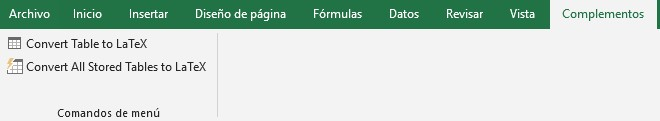
\includegraphics[width=.9\linewidth]{complementos_excel.jpg}
     \caption{Complemento excel2latex en Excel}
\end{figure}

Simplemente habrá que seleccionar una tabla en \textit{Excel}, y a continuación clicar en \texttt{Convert Table To LaTeX} que resultará en una nueva ventana con el código en el que se puede copiar e incluso realizar otro tipo de acciones.\newline

Por último, destacar que la licencia por la que se rige es \textit{The LaTeX Project Public Li­cense 1.3} y que a pesar de que no se identifica el autor del copyright, como mantenimiento se encuentran Chelsea Hughes y Kir­ill Müller.

\subsection*{Ejemplos de cómo hacer figuras}

\paragraph*{Ejemplo de dos figuras lado a lado}

\begin{figure}[H]
   \begin{minipage}{0.45\textwidth}
     \centering
     
\includegraphics[width=.6\linewidth]{LogoGuardMe}
     \caption{Figura izquierda}
     \label{fizq1}
   \end{minipage}
   \hfill
   \begin{minipage}{0.45\textwidth}
     \centering
     
\includegraphics[width=.6\linewidth]{LogoGuardMe}
     \caption{Figura derecha}
     \label{fdcha1}
   \end{minipage}
\end{figure}


\paragraph*{Ejemplo de figura}

\begin{figure}[H]
     \centering
     
\includegraphics[width=.2\linewidth]{LogoGuardMe}
     \caption{Figura de ejemplo}
     \label{fig1}
\end{figure}

\subsection*{Listas de items}

\paragraph*{Lista de items estándar}
 
\renewcommand{\labelitemi}{$-$}
\begin{itemize}
  \item El \textbf{uso de la aplicación} por parte de una gran cantidad de usuarios \textbf{sin importar el sistema operativo} del que dispongan.
  \item La posibilidad de realizar una \textbf{llamada a emergencias al (\textit{112})de manera rápida e intuitiva}, al mismo tiempo que se avisa a los protectores del usuario que solicite auxilio.
  \item La \textbf{monitorización de localización} por parte de los protectores de los usuarios que posean como protegidos.
  \item La \textbf{comunicación entre protector y protegido} a través de un servicio de mensajería dentro de la aplicación.
\end{itemize}

\paragraph*{Lista estándar multinivel}

\begin{itemize}
	\item Prueba: el usuario se registrar por primera vez en la aplicación.
	\item Resultados
	\begin{itemize}
		\item Esperado: el usuario aparece tanto en la lista de usuarios registrados de Firebase Authentication como en la base de datos de la aplicación.
		\item Obtenido: el usuario parece inscrito en ambos registros.
	\end{itemize}
\end{itemize}

\paragraph*{Lista multinivel para Ingeniería de Requisitos}

\newlist{myEnumerate}{enumerate}{9}
\setlist[myEnumerate,1]{label=\textbf{RF-\arabic*.}}
\setlist[myEnumerate,2]{label*=\textbf{\arabic*.}}
\setlist[myEnumerate,3]{label*=\textbf{\arabic*.}}
\setlist[myEnumerate,4]{label*=\textbf{\arabic*.}}
\setlist[myEnumerate,5]{label*=\textbf{\arabic*.}}
\setlist[myEnumerate,6]{label*=\textbf{\arabic*.}}
\setlist[myEnumerate,7]{label*=\textbf{\arabic*.}}
\setlist[myEnumerate,8]{label*=\textbf{\arabic*.}}
\setlist[myEnumerate,9]{label*=\textbf{\arabic*.}}

\newlist{myEnumNF}{enumerate}{4}
\setlist[myEnumNF,1]{label=\textbf{RNF-\arabic*.}}
\setlist[myEnumNF,2]{label*=\textbf{\arabic*.}}
\setlist[myEnumNF,3]{label*=\textbf{\arabic*.}}
\setlist[myEnumNF,4]{label*=\textbf{\arabic*.}}

\subsubsection*{Requisitos funcionales}
\paragraph*{Registro e inicio de sesión}

\begin{myEnumerate}
  \item Un usuario deberá poder registrarse en el sistema.\label{req_registro} %RF-1
  \begin{myEnumerate}
    
    \item Un usuario deberá registrarse con unas credenciales pertenecientes a una cuenta de Google.
    \begin{myEnumerate}
      \item El sistema no permitirá que un usuario se registre más de una vez.
      \item El sistema pedirá la confirmación de los credenciales a Google.
      \begin{myEnumerate}
      	\item En caso de que los credenciales sean correctos, se accederá a la aplicación por primera vez.
      	\item En caso de que los credenciales sean erróneos, se informará al usuario de dicho error.
       \end{myEnumerate}
    \end{myEnumerate}
    
    \item Un usuario deberá proporcionar el número de teléfono correspondiente al dispositivo que esté utilizando.
    \begin{myEnumerate}
    	\item El sistema comprobará que el número de teléfono corresponde al dispositivo con el que se esté realizando el registro.
    	\begin{myEnumerate}
     		\item El sistema emitirá un mensaje SMS a dicho dispositivo que se detectará automáticamente.
      		\item El sistema validará el código de SMS recibido con el de la base de datos.
    	\end{myEnumerate}
   	\end{myEnumerate} 
   	
   	\item Una vez finalizado el registro, el sistema automáticamente:
   		\begin{myEnumerate}
   		\item Escribirá los datos recibidos del registro en la base de datos:
    		\begin{myEnumerate}
      			\item Nombre
      			\item Apellidos
      			\item Email
      			\item Número de teléfono
      			\item UID de Google
      			\item URL de la imagen de perfil
      			\item Locale
      			\item Fecha de creación
      			\item Fecha de último inicio de sesión
    		\end{myEnumerate}
    		
    	\item Redirigirá al usuario a la pantalla principal.
    	\end{myEnumerate}
  \end{myEnumerate}
  
  \item Un usuario deberá poder iniciar sesión en el sistema. %RF-2
    \begin{myEnumerate}%RF2.1
      \item Un usuario deberá iniciar sesión mediante las credenciales de Google.
      \begin{myEnumerate}%RF2.1.1
      	\item El sistema comprobará que las credenciales sean correctas.
      	\item El sistema verificará que el usuario existe en la base de datos.
      		\begin{myEnumerate}%RF2.1.1.1
      			\item En caso de no existir, el sistema automáticamente:
      			\begin{myEnumerate}%RF2.1.1.1.1
      				\item Registrará al usuario siguiendo \textit{\ref{req_registro}}.
      				\item Notificará a usuario.
      			\end{myEnumerate}
      			\item En caso de existir, el sistema automáticamente actualizará la información del usuario en la base de datos:
      			\begin{myEnumerate}
      				\item Fecha de último inicio de sesión
      			\end{myEnumerate}
      		\end{myEnumerate}
      \end{myEnumerate}
      
      \item Una vez finalizado el inicio de sesión, el sistema automáticamente redirigirá al usuario a la pantalla principal.
    \end{myEnumerate}
\end{myEnumerate}

\paragraph*{Llamada de emergencia}

\begin{myEnumerate}[resume*]
  \item Un usuario deberá poder realizar una llamada de auxilio.
  \begin{myEnumerate}
    \item El usuario deberá tener la sesión iniciada en la aplicación.
  	\item Un usuario podrá clicar en un botón para realizar en la llamada.
  	\begin{myEnumerate}
  		\item El sistema verificará que la llamada no ha sido sin querer.
  		\begin{myEnumerate}
  			\item En caso de haber sido voluntaria, el sistema automáticamente realizará una llamada telefónica al teléfono de emergencias 112.
  				\begin{myEnumerate}
  					\item Los gastos de la llamada se atribuirán a cargo del usuario.
				\end{myEnumerate}
  			\item En caso de haber sido voluntaria, el sistema automáticamente realizará un aviso a los protectores del usuario en caso de tenerlos.
  				\begin{myEnumerate}
  					\item El sistema guardará la última ubicación registrada.
  					\item El sistema generará una alerta a los protectores que contenga los siguientes datos del usuario:
					 \begin{myEnumerate}
  						\item Nombre
  						\item Apellidos
  						\item Última localización registrada
  					 \end{myEnumerate}
			    \end{myEnumerate}
  		\end{myEnumerate}
  	\end{myEnumerate}
  	\item El sistema proporcionará un botón fácil de ver y clicar.
  \end{myEnumerate}
\end{myEnumerate}

\subsubsection*{Requisitos no funcionales}
\begin{myEnumNF}
	\item El usuario deberá ser capaz de utilizar todas las funcionalidades desarrolladas en la aplicación sin problema.
	\item La aplicación sera accesible para los usuarios a través de un portal de descarga.
	\begin{myEnumNF}
		\item La aplicación será multiplataforma.
		\begin{myEnumNF}
			\item La aplicación requiere mínimo las versiones:
			\begin{myEnumNF}
				\item 5.0 para Android
				\item 10.0 para iOS
			\end{myEnumNF}
			\item Las versiones están condicionadas por los requisitos de Expo.
		\end{myEnumNF}
	\end{myEnumNF}
	
	\item Los servicios que utiliza la aplicación deberán mantenerla disponible el mayor tiempo posible.
	\begin{myEnumNF}
		\item El sistema estará disponible siguiendo el protocolo de los tres nueves: 99.9\%.
		\begin{myEnumNF}
			\item El sistema no estará disponible 43,8 minutos/mes u 8,76 horas/año.
		\end{myEnumNF}
	\end{myEnumNF}
	\item Los usuarios de la aplicación no deberán tener conocimientos tecnológicos avanzados.
		\begin{myEnumNF}
		\item El nivel básico será requerido, lo que incluye haber tratado con un teléfono móvil alguna vez.
	\end{myEnumNF}
	
	\item El sistema se conectará con la base de datos que albergará todos los datos asociados a los usuarios registrados y sus datos.
	\begin{myEnumNF}
		\item Las base de datos estará alojada en la nube.
		\item Los tiempos de carga de datos no deberán sobrepasar los 10 segundos.
	\end{myEnumNF}

	\item El sistema se comunicará con:
	\begin{myEnumNF}
		\item Google Maps API
		\item Google Firebase Cloud Firestore
		\item Google Firebase Authentication
		\item Whatsapp
	\end{myEnumNF}
\end{myEnumNF}


\subsection*{Ejemplos de cómo hacer tablas}

\paragraph*{Tabla descripción clases}

\begin{table}[H]
  \centering
  \caption{Análisis de LoginScreen}
    \begin{tabular}{p{8.645em}rr}
    \toprule
    \rowcolor[rgb]{ .851,  .886,  .953} \multicolumn{3}{p{31.285em}}{\textbf{LoginScreen}} \\
    \midrule
    \rowcolor[rgb]{ .949,  .949,  .949} \multicolumn{3}{p{31.285em}}{\textbf{Descripción}} \\
    \midrule
    \multicolumn{3}{p{31.285em}}{Es la encargada de las acciones y la renderización de la pantalla de inicio de sesión.} \\
    \midrule
    \rowcolor[rgb]{ .906,  .902,  .902} \multicolumn{3}{p{31.285em}}{\textbf{Atributos propuestos}} \\
    \midrule
    \multicolumn{3}{p{31.285em}}{-} \\
    \midrule
    \rowcolor[rgb]{ .906,  .902,  .902} \multicolumn{3}{p{31.285em}}{\textbf{Métodos propuestos}} \\
    \midrule
    \textbf{componentWillMount} & \multicolumn{2}{r}{} \\
    \midrule
    \textbf{signIn} & \multicolumn{2}{p{22.64em}}{Inciar sesión en Firebase} \\
    \midrule
    \textbf{render} & \multicolumn{2}{r}{} \\
    \bottomrule
    \end{tabular}%
    \vspace{-4mm}
\end{table}%


\paragraph*{Tabla típica}

\begin{table}[H]
  \centering
  \caption{Planificación de Formación}
    \begin{tabular}{p{5.355em}p{14.785em}p{6.07em}}
    \toprule
    \textbf{Num. esq.} & \textbf{Nombre de tarea} & \textbf{Duración} \\
    \midrule
    \textbf{1.1} & \textbf{Formación propia} & \textbf{34 horas} \\
    \midrule
    \textit{1.1.1} & \textit{   Aprender sobre Expo} & \textit{19,5 horas} \\
    \textit{1.1.2} & \textit{   Aprender sobre React-Native} & \textit{8 horas} \\
    \textit{1.1.3} & \textit{   Aprender sobre base de datos} & \textit{16,5 horas} \\
    \textit{1.1.4} & \textit{   Aprender sobre Typescript} & \textit{3 horas} \\
    \textit{1.1.5} & \textit{   Aprender sobre Scaledrone} & \textit{3 horas} \\
    \textit{1.1.6} & \textit{   Aprender sobre LaTeX} & \textit{5,5 horas} \\
    \bottomrule
    \end{tabular}
\end{table}%

\paragraph*{Tabla ejemplo para especificar un presupuesto}

\begin{table}[H]
  \centering
  \caption{Resumen del presupuesto}
    \begin{tabular}{rrr}
    \toprule
    \multicolumn{1}{c}{\textbf{COD.}} & \multicolumn{1}{c}{\textbf{Descripción}} & \multicolumn{1}{c}{\textbf{Subtotal}} \\
    \midrule
    \multicolumn{1}{c}{\textit{001}} & \multicolumn{1}{l}{\textit{Formación}} & \textit{\EUR{1.110,00}} \\
    \midrule
    \multicolumn{1}{c}{\textit{002}} & \multicolumn{1}{l}{\textit{Estudio de Alternativas}} & \textit{\EUR{400,00}} \\
    \midrule
    \multicolumn{1}{c}{\textit{003}} & \multicolumn{1}{l}{\textit{Análisis y Diseño}} & \multicolumn{1}{c}{\textit{ \EUR{1.840,00}}} \\
    \midrule
    \multicolumn{1}{c}{\textit{004}} & \multicolumn{1}{l}{\textit{Desarrollo}} & \multicolumn{1}{c}{\textit{ \EUR{10.860,00}}} \\
    \midrule
    \multicolumn{1}{c}{\textit{005}} & \multicolumn{1}{l}{\textit{Documentación}} & \multicolumn{1}{c}{\textit{ \EUR{3.985,00}}} \\
    \midrule
    \multicolumn{2}{r}{\textit{\textbf{TOTAL}}} & \textbf{ \EUR{18.195,00}} \\
    \bottomrule
    \end{tabular}
\end{table}%

\subsection*{Otros elementos}

\paragraph*{URLs}

\url{www.javascript.com/learn/}

\paragraph*{Fracciones}

El portátil se trata de un Lenovo 80E5 i7 con 8 GB RAM y con 4 años de uso, el cual costó entonces \EUR{650}, por lo tanto la amortización será de \EUR{26} al año según:

\[\dfrac{650 - 545}{4} 
  \equiv 26
\]

\end{document}